Now we are ready to investigate the effects of the different choices of the algorithm parameter $\Delta$ on the thermalization speed and autocorrelation time of the chain.
The first concept we need to introduce is the acceptance.

The proposal for an updated coordinate (equation \ref{eqn:proposal}) selects an $x_{i}'$ inside a closed interval of center
$x_{i}$ and width $\Delta$: it is reasonable that such parameter influences the efficiency of the Metropolis
algorithm. We define \textit{acceptance rate} or simply \textit{acceptance} the frequency of a new proposal getting accepted.

\begin{figure}[h!]
  \centering
 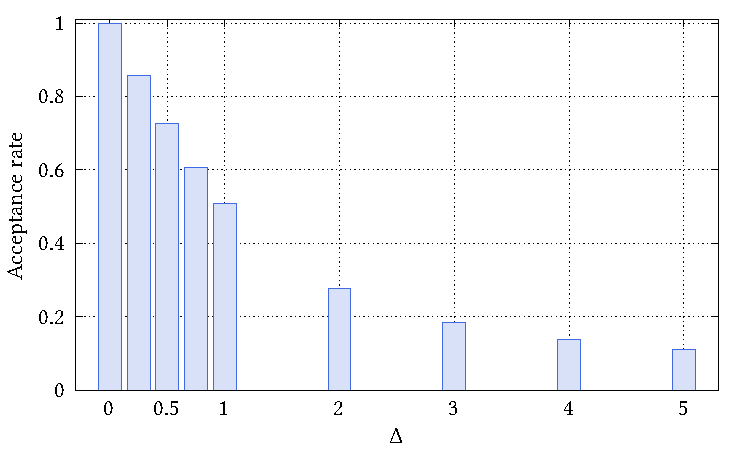
\includegraphics[width=\linewidth]{accettanza}
  \caption{\label{fig:acceptance} Acceptance rate plotted against the value of $\Delta$. Acceptance decreases for larger $\Delta$ values. }
\end{figure}

The higher the acceptance, the more likely it is that a new proposal is accepted, which is desirable from a computational
cost standpoint since it implies less \textit{void} iterations of the algorithm. On the other hand, the purpose of the Metropolis algorithm
is to iteratively refine the transition probability of a Markov chain, therefore we would like a somewhat strict selection.
Figure \ref{fig:acceptance} gives some insight on the acceptance rate for different values of $\Delta$.

The limit case with $\Delta = 0$, $\text{acceptance}=1$, is a good example of the concept above: if $\Delta = 0$, every sweep would be an exact copy of the previous
so the chain will never reach the desired thermalization value.

\begin{figure}[ht]
  \centering
  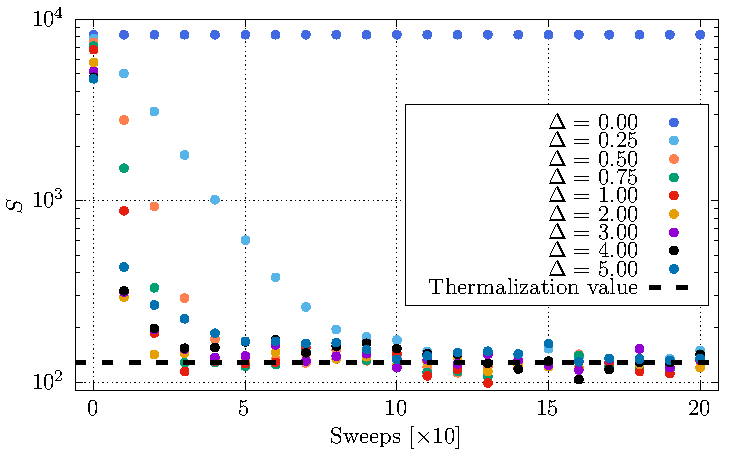
\includegraphics[width=\linewidth]{thermdelta}
  \caption{\label{fig:thermdelta}Thermalization speed for different values of $\Delta$. The action is plotted once every $10$ sweeps. If $\Delta \neq 0$, the thermalization value
  is reached with variable speed: the sweet spot seems to be around $1\le \Delta \le 3$.}
\end{figure}

Figure \ref{fig:thermdelta} shows the values of the action as a function of Markovian time, plotted once every $10$ sweeps, for different values
of $\Delta$. The thermalization time decreases up to $\Delta = 3$ and then it starts slowly growing again.

Since the composition of each configuration heavily depends on $\Delta$,
the parameter also influences the autocorrelation time $\tau_{int}$.
This dependence is analyzed in figure \ref{fig:taudelta}.
\begin{figure}[h!]
  \centering
  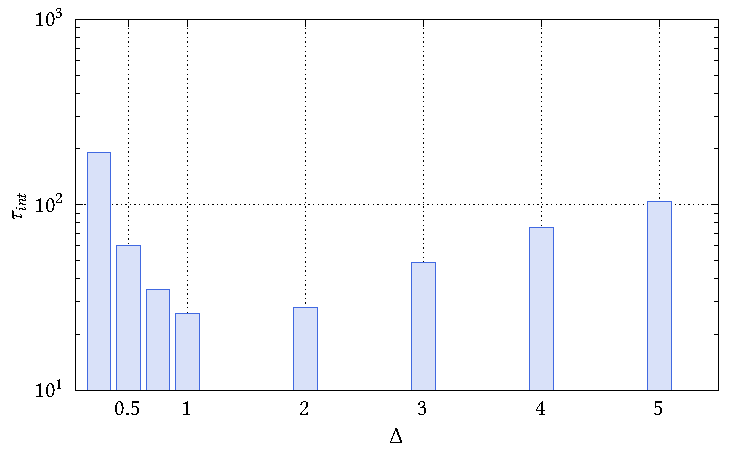
\includegraphics[width=\linewidth]{tau}
  \caption{\label{fig:taudelta}Interaction time in $\log$ scale for different values of $\Delta$. $\Delta = 0$ is not considered as every
  sweep simply copies the previous.}
\end{figure}

The interaction time decreases from $\Delta = 0.25$ to $\Delta = 1$, where it reaches its minimum, then starts growing again: this is
the parameter we decided to prioritize. Autocorrelation time is used to determine the dimension of each bin and, as a consequence, the number of
of bins for a fixed number of sweeps. In order to maximize the number of bins, we kept $\Delta = 1$ for the entire simulation.
